%%%%%%%%%%%%%%%%%%%%%%%%%%%%%%%%%%%%%%%%%%%%%%%%%%%%%%%%%%%%%%%%%%%%%%%%%%%%%%%%%%%%%%%%%%%%%%%%%%%%%%%%%%%%%%%%%%%%%%%%%%%%%%%%%%%%%%%%%%%%%%%%%%%%%%%%%%%
% This is just an example/guide for you to refer to when submitting manuscripts to Frontiers, it is not mandatory to use Frontiers .cls files nor frontiers.tex  %
% This will only generate the Manuscript, the final article will be typeset by Frontiers after acceptance.   
%                                              %
%                                                                                                                                                         %
% When submitting your files, remember to upload this *tex file, the pdf generated with it, the *bib file (if bibliography is not within the *tex) and all the figures.
%%%%%%%%%%%%%%%%%%%%%%%%%%%%%%%%%%%%%%%%%%%%%%%%%%%%%%%%%%%%%%%%%%%%%%%%%%%%%%%%%%%%%%%%%%%%%%%%%%%%%%%%%%%%%%%%%%%%%%%%%%%%%%%%%%%%%%%%%%%%%%%%%%%%%%%%%%%

%%% Version 3.3 Generated 2016/11/10 %%%
%%% You will need to have the following packages installed: datetime, fmtcount, etoolbox, fcprefix, which are normally inlcuded in WinEdt. %%%
%%% In http://www.ctan.org/ you can find the packages and how to install them, if necessary. %%%
%%%  NB logo1.jpg is required in the path in order to correctly compile front page header %%%

\documentclass[utf8]{frontiersSCNS} % for Science, Engineering and Humanities and Social Sciences articles
%\documentclass[utf8]{frontiersHLTH} % for Health articles
%\documentclass[utf8]{frontiersFPHY} % for Physics and Applied Mathematics and Statistics articles

%\setcitestyle{square} % for Physics and Applied Mathematics and Statistics articles
\usepackage{url,hyperref,lineno,microtype,subcaption}
\usepackage[onehalfspacing]{setspace}
\hypersetup{hidelinks=true}    
\usepackage{xcolor}
\linenumbers


% Leave a blank line between paragraphs instead of using \\


\def\keyFont{\fontsize{8}{11}\helveticabold }
\def\firstAuthorLast{Ramele {et~al.}} %use et al only if is more than 1 author
\def\Authors{Rodrigo Ramele\,$^{1,*}$, Ana Julia Villar\,$^{1}$ and Juan Miguel Santos\,$^{1}$}
% Affiliations should be keyed to the author's name with superscript numbers and be listed as follows: Laboratory, Institute, Department, Organization, City, State abbreviation (USA, Canada, Australia), and Country (without detailed address information such as city zip codes or street names).
% If one of the authors has a change of address, list the new address below the correspondence details using a superscript symbol and use the same symbol to indicate the author in the author list.
\def\Address{$^{1}$Centro de Inteligencia Computacional, Computer Engineering Department,\\ 
Instituto Tecnológico de Buenos Aires(ITBA), Buenos Aires, Argentina}
% The Corresponding Author should be marked with an asterisk
% Provide the exact contact address (this time including street name and city zip code) and email of the corresponding author
\def\corrAuthor{Rodrigo Ramele, C1437FBH Lavarden 315, Ciudad Autónoma de Buenos Aires, Argentina}

\def\corrEmail{rramele@itba.edu.ar}

\begin{document}
\onecolumn
\firstpage{1}

\title[Histogram of Gradient Orientations of Signal Plots]{Histogram of Gradient Orientations of Signal Plots applied to P300 Detection} 

\author[\firstAuthorLast ]{\Authors} %This field will be automatically populated
\address{} %This field will be automatically populated
\correspondance{} %This field will be automatically populated

\extraAuth{}% If there are more than 1 corresponding author, comment this line and uncomment the next one.
%\extraAuth{corresponding Author2 \\ Laboratory X2, Institute X2, Department X2, Organization X2, Street X2, City X2 , State XX2 (only USA, Canada and Australia), Zip Code2, X2 Country X2, email2@uni2.edu}


\maketitle


\begin{abstract}

%%% Leave the Abstract empty if your article does not require one, please see the Summary Table for full details.
\section{}
Word Count: 5552 \\
The analysis of Electroencephalographic (EEG) signals is of ulterior importance to aid in the diagnosis of mental disease and to increase our understanding of the brain.  Traditionally, clinical EEG has been analyzed in terms of temporal waveforms, looking at rhythms in spontaneous activity, subjectively identifying troughs and peaks in Event-Related Potentials (ERP), or by studying graphoelements in pathological sleep stages.
Additionally, the discipline of Brain Computer Interfaces requires new methods to decode patterns from non-invasive EEG signals.  This field is developing alternative communication pathways to transmit volitional information from the Central Nervous System. The technology could potentially enhance the quality of life of patients affected by neurodegenerative disorders and other mental illness. This work mimics what electroencephalographers have been doing clinically, visually inspecting and categorizing phenomena within the EEG by the extraction of features from images of signal plots.  These features are constructed based on the calculation of histograms of oriented gradients from pixels around the signal plot. It aims to provide a new objective framework to analyze, characterize and classify EEG signal waveforms. The feasibility of the method is outlined by detecting the P300, an ERP elicited by the oddball paradigm of rare events, and implementing an offline P300-based BCI Speller.  The validity of the proposal is shown by offline processing a public dataset of Amyotrophic Lateral Sclerosis (ALS) patients and an own dataset of healthy subjects.

\tiny
 \keyFont{ \section{Keywords:} electroencephalography, histogram of gradient orientations, brain-computer interfaces, P300, SIFT, amyotrophic lateral sclerosis, naive-bayes near neighbours, waveforms} %All article types: you may provide up to 8 keywords; at least 5 are mandatory.
\end{abstract}

\section{Introduction}

%The EEG is traditionally analyzed in terms of temporal waveforms at certain channels, looking at power of rhythms in the spontaneous EEG, at amplitude and latency of the peaks and troughs in event- related potentials (ERPs), or at particular grapho-elements in patho- logical or sleep stages.

Although recent advances in neuroimagining techniques, particularly radio-nuclear and radiological scanning methods \citep{Schomer2010}, have diminished the prospects of the traditional Electroencephalography (EEG), the advent and development of digitized devices has impelled for a revamping of this hundred years old technology.  Their versatility, ease of use, temporal resolution, ease of development and production, and its proliferation as consumer devices, are pushing EEG to become the de-facto non invasive portable or ambulatory method to access and harness brain information~\citep{DeVos2014}.

A key contribution to this expansion has been the field of Brain Computer Interfaces (BCI)~\citep{WolpawJonathanR2012} which is the pursuit of the development of a new channel of communication particularly aimed to persons affected by neurodegenerative diseases.

One noteworthy aspect of this novel communication channel is the ability to transmit information from the Central Nervous System (CNS) to a computer device and from there use that information to control a wheelchair~\citep{Carlson2013}, as input to a speller application~\citep{Guger2009a}, in a Virtual Reality environment~\citep{Lotte2013} or as aiding tool in a rehabilitation procedure~\citep{Jure2016}.  The holly grail of BCI is to implement a new complete and alternative pathway to restore lost locomotion~\citep{WolpawJonathanR2012}.

EEG signals are remarkably complex and have been characterized as a multichannel non-stationary stochastic process.  Additionally, they have high variability between different subjects and even between different moments for the same subject, requiring adaptive and co-adaptive calibration and learning procedures~\citep{Clerc}.  Hence, this imposes an outstanding challenge that is necessary to overcome in order to extract information from raw EEG signals.

%Moreover, EEG markers~\citep{Clerc} that can be used to  transmit volitional information are limited, and each one of them has a particular combination of appropriate methods to decode them. Inevitably, it is necessary to implement  distinct and specialized algorithmic methods, to filter the signal, enhance its Signal to Noise Ratio (SNR), and try to determine some meaning out of it.  

BCI has gained mainstream public awareness with worldwide challenge competitions like Cybathlon~\citep{Riener2014,cybathlon2} and even been broadcasted during the inauguration ceremony of the 2014 Soccer World Cup.  New developments have overcome the out-of-the-lab high-bar and they are starting to be used in real world environments~\citep{Guger2017,Huggins2016}.  However, they still lack the necessary robustness, and its performance is well behind any other method of human computer interaction, including any kind of detection of residual muscular movement~\citep{Clerc}.

A few works have explored the idea of exploiting the signal waveform to analyze the EEG signal.  In~\citep{Alvarado-Gonzalez2016} an approach based on Slope Horizontal Chain Code is presented, whereas in~\citep{Yamaguchi2009} a similar procedure was implemented based on Mathematical Morphological Analysis.  The seminal work of Bandt-Pompe Permutation Entropy~\citep{Berger2017} also explores succinctly this idea as a basis to establish the time series ordinal patterns.  In the article~\citep{Ramele2016},  the authors introduce a method for classification of rhythmic EEG events like Visual Occipital Alpha Waves  and Motor Imagery Rolandic Central $\mu$ Rhythms using the Histogram of Gradient Orientations of signal plots.  Inspired in that work, we propose a novel application of the developed method to classify and describe transient events, particularly the P300 Event Related Potential.  
The proposed approach is based on the waveform analysis of the shape of the EEG signal.  The signal is drawn on a bidimensional image plot, vector gradients of pixels around the plot are obtained, and with them, the histogram of their orientations is calculated.  This histogram is a direct representation of the waveform of the signal. The method is built by mimicking what regularly electroencephalographers have been performing for almost a century as it is described in~\citep{Hartman2005}: visually inspecting raw signal plots.

This paper reports a method to, (1) describe a procedure to capture the shape of a waveform of an ERP component, the P300, using histograms of gradient orientations extracted from images of signal plots, and (2) outline the way in which this procedure can be used to implement an P300-Based BCI Speller application. Its validity is verified by offline processing two datasets, one of data from ALS patients and another one from data of healthy subjects. 

This article unfolds as follows: Section~\ref{Feature} is dedicated to explain the Feature Extraction method based on Histogram of Gradient Orientations of the Signal Plot: Section~\ref{Pipeline} shows the preprocessing pipeline,  Section~\ref{Plot}  describes the image generation of the signal plot, Section~\ref{SIFT}  presents the feature extraction procedure while  Section~\ref{Classification}  introduces the Speller Matrix Letter Identification procedure.  In Section~\ref{Protocol}, the experimental protocol is expounded. Section~\ref{Results} shows the results of applying the proposed technique.  In the final Section~\ref{discussion}  we expose our remarks, conclusions and future work.

\section{Materials and Methods}

The P300~\citep{Farwell1988,Knuth2006} is a positive deflection of the EEG signal which occurs around $300$ ms after the onset of a rare and deviant stimulus that the subject is expected to attend.  It is produced under the oddball paradigm~\citep{WolpawJonathanR2012} and it is consistent across different subjects. It has a lower amplitude  ($\pm 5 \mu V $) compared to basal EEG activity, reaching a Signal to Noise Ratio (SNR) of around $-15$ db estimated based on the amplitude of the P300 response signal divided by the standard deviation of the background EEG activity~\citep{Hu2010}.  This signal can be used to implement a speller application by means of a Speller Matrix~\citep{Farwell1988}. This matrix is composed of 6 rows and 6 columns of numbers and letters. The subject can focus on one character of the matrix. Figure~\ref{fig:p300matrix} shows an example of the Speller Matrix used in the OpenVibe open source software~\citep{Renard2010}, where the flashes of rows and columns provide the deviant stimulus required to elicit this physiological response.   Each time a row or a column that contains the desired letter flashes, the corresponding synchronized EEG signal should also contain the P300 signature and by detecting it, the selected letter can be identified.

\subsection{Feature Extraction from Signal Plots} \label{Feature}

In this section, the signal preprocessing, the method for generating images from signal plots, the feature extraction procedure and the Speller Matrix identification are described.  Figure~\ref{fig:classification} shows a scheme of the entire process.

\subsubsection{Preprocessing Pipeline} \label{Pipeline}

The data obtained by the capturing device is digitalized and a multichannel EEG signal is constructed.

%A trial, as defined by the BCI2000 platform~\citep{Schalk2004}, is every attempt to select a letter from the speller. 

%It is composed of signal segments $S_{i}^l$ corresponding to $k_a$ repetitions of flashes of 6 rows and $k_a =10$ repetitions of flashes of 6 columns of the matrix, yielding 120 repetitions. 

The $6$ rows and $6$ columns of the Speller Matrix are intensified providing the visual stimulus.  The number of a row or column is a location. A sequence of twelve randomly permuted locations $l$ conform an intensification sequence. The whole set of twelve intensifications is repeated $k_a$ times.

%The multichannel EEG signal is processed on a channel by channel basis.   

\begin{itemize}
\item \textbf{Signal Enhancement}: This stage consists of the enhancement of the SNR of the P300 pattern above the level of basal EEG. The pipeline starts by applying a notch filter to the raw digital signal, a $4$th degree $10$ Hz lowpass Butterworth filter and finally a decimation with a Finite Impulse Response (FIR) filter of order $30$ from the original sampling frequency down to $16$ Hz \citep{Krusienski2006}.
\item \textbf{Artifact Removal}: For every complete sequence of $12$ intensifications of $6$ rows and $6$ columns, a basic artifact elimination procedure is implemented by removing the entire sequence when any signal deviates above/bellow $ \pm 70 \mu V $.
\item \textbf{Segmentation}: For each of the $12$ intensifications of one intensification sequence,  a segment $S_{i}^l$  of a window of $t_{max} $ seconds of the multichannel signal is extracted, starting from the stimulus onset, corresponding to each row/column intensification $l$ and to the intensification sequence $i$. As intensifications are permuted in a random order, the segments are rearranged corresponding to row flickering, labeled 1-6, whereas those corresponding to column flickering are labeled 7-12.  Two of these segments should contain the P300 ERP signature time-locked to the flashing stimulus, one for the row, and one for the column.
\item \textbf{Signal Averaging}: \label{Average}  The P300 ERP is deeply buried under basal EEG so the standard approach to identify it is by point-to-point averaging the time-locked stacked signal segments.  Hence the values which are not related to, and not time-locked to the onset of the stimulus are canceled out~\citep{Liang2008}.  

This last step determines the operation of any P300 Speller.  In order to obtain an improved signal in terms of its SNR,  repetitions of the sequence of row/column intensification are necessary.  And, at the same time, as long as more repetitions are needed, the ability to transfer information faster is diminished, so there is a trade-off that must be acutely determined.

The procedure to obtain the point-to-point averaged signal goes as follows:

\begin{enumerate}
\item \label{paso1}Highlight randomly the rows and columns from the matrix.  There is one row and one column that should match the letter selected by the subject.
\item  \label{paso2} Repeat step~\ref{paso1} $k_a$ times, obtaining the $1 \leq l \leq 12$ segments $S_1^l(n,c),\dots,S_{k_a}^l(n,c)$, of the EEG signal where the variables $1 \leq n \leq n_{max}$ and $1 \leq c \leq C$  correspond to sample points and channel, respectively. The parameter $C$ is the number of available EEG channels whereas $n_{max}=F_s \  t_{max}$ is the segment length and $F_s$ is the sampling frequency.  The parameter $k_a$ is the number of repetitions of intensifications and it is an input parameter of the algorithm.
\item \label{paso3} Compute the Ensemble Average by
\begin{equation}
x^l(n,c)= \frac{1}{k_a}\sum_{i=1}^{k_a}S_i^l(n,c) 
\label{averaging}
\end{equation}  
for $1 \leq n \leq n_{max}$ and for the channels $1 \leq c \leq C$.  This provide an averaged signal $x^l(n,c)$ for the twelve locations $ 1 \leq l \leq 12$.
\end{enumerate}
\end{itemize}

\subsubsection{Signal Plotting} \label{Plot}

Averaged signal segments are standardized and scaled for $1 \leq n \leq n_{max}$ and $1 \leq c \leq C$ by 

\begin{equation}
\tilde{x}^l(n,c) = \left \lfloor{ \gamma \; \frac{( x^l(n,c) - \bar{x}^l(c)  )}{ \hat{\sigma}^l(c) } }\right \rfloor
\label{eq:standarizedaverages}
\end{equation}

\noindent where $\gamma > 0$ is an input parameter of the algorithm and  it is related to the image scale. In addition, $ x^l(n,c) $ is the point-to-point averaged multichannel EEG signal for the sample point $n$ and for channel $c$. Lastly, $$\bar{x}^l(c) =\frac{1}{n_{max}}\sum_{n=1}^{n_{max}}x^l(n,c)$$ and $$ \hat{\sigma}^l(c) =  \bigg \{  \frac{1}{n_{max}-1}\sum_{n=1}^{n_{max}} { \left[  x^l(n,c)-\bar{x}^l(c)  \right]  }^2 \bigg \} ^{\frac{1}{2}}$$ are the mean and estimated standard deviation of $x^l(n,c), 1 \leq n \leq n_{max}$, for each channel $c$.

Consequently, a binary image $I^{(l,c)}$ is constructed according to


\begin{equation}
I^{(l,c)}(z_1,z_2) = \left\{ \begin{array}{rl}
255 & \text{if} \;  z_1 = \gamma \  n \quad \text{and}  \quad  \! z_2 = \tilde{x}^l(n,c) + z^l(c) \\
0   & \mbox{otherwise}
\end{array}\right.
\label{eq:images}
\end{equation}

\noindent with $255$ being white and representing the signal's value location and $0$ for black which is the background contrast, conforming a black-and-white plot of the signal.  Pixel arguments $ (z_1,z_2) \in \mathbb{N} \times \mathbb{N}$ iterate over the width (based on the length of the signal segment) and height (based on the peak-to-peak amplitude) of the newly created image with $1 \leq n \leq n_{max}$ and $1 \leq c \leq C$.  The value $z^l(c)$ is the image vertical position where the signal's zero value has to be situated in order to fit the entire signal within the image for each channel c:

\begin{equation}
z^l(c) = \left \lfloor{ \frac{\max_{n} \tilde{x}^l(n,c)  - \min_{n} \tilde{x}^l(n,c) }{2} }\right \rfloor -   \left \lfloor{ \frac{\max_{n} \tilde{x}^l(n,c)  + \min_{n} \tilde{x}^l(n,c)}{ 2} }\right \rfloor
\label{eq:zerolevel}
\end{equation}

\noindent where the minimization and maximization are carried out for $n$ varying between ${1 \leq n\leq n_{max}}$, and $ \lfloor \cdot  \rfloor $ denote the rounding to the smaller nearest integer of the number.
  
In order to complete the plot $I^{(l,c)}$ from the pixels, the Bresenham \citep{Bresenham1965,Ramele2016} algorithm is used to interpolate straight lines between each pair of  consecutive pixels.


\subsubsection{Feature Extraction: Histogram of Gradient Orientations}
\label{SIFT}

The work of Edelman, Intrator and Poggio~\citep{cogprints561} on how the visual cortex sense features was the inspiration to the development of an algorithm to identify and decode salient local information from image regions.  The Scale Invariant Feature Transform (SIFT) is a Computer Vision method proposed by~\cite{Lowe2004} which is composed of two parts, the SIFT Detector and the SIFT Descriptor.  The former is the procedure to identify relevant areas of an image whereas the latter is the procedure to describe and characterize a region of an image (i.e. patch) calculating an histogram on the angular orientations of pixel gradients.  In order to characterize EEG signal waveforms, this work proposes an alternative to the SIFT Descriptor, the Histogram of Gradient Orientations algorithm.  

%We stripped away all the details which are not used and refined the procedure to enable the effective capturing of the waveform shape.

%Aca sacar la parte que detalla de que se sacaron los detalles de SIFT

For each generated image $I^{(l,c)}$, a keypoint $\mathbf{p_k}$ is placed on a pixel $(x_{p_k}, y_{p_k})$ over the image plot and a window around the keypoint is considered. A local image patch of size $X_p \times X_p$ pixels is constructed by dividing the window in $16$ blocks of size $3s$ each one,  where $s$ is the scale of the local patch and it is an input parameter of the algorithm. It is arranged in a $4 \times 4$ grid and the pixel $ \mathbf{p_k}$ is the patch center, thus $X_p = 12s $ pixels. 

A local representation of the signal shape within the patch can be described by obtaining the gradient orientations on each of the $16$ blocks $B_{i,j}$  with $ 0 \leq i,j \leq 3$ and creating a histogram of gradients.  In order to calculate the histogram, the interval $[0,360]$ of possible angles is divided in $8$ bins, each one of $45$ degrees.

 Hence, for each spatial bin $ 0 \leq i,j \leq 3$, corresponding to the indexes of each block $B_{i,j}$,  the orientations are accumulated in a  $3$-dimensional histogram $h$ through the following equation: 
 

\begin{equation}
 h(\theta,i,j) = 3 s \sum_{\mathbf{p} \in I^{(l,c)}} w_\mathrm{ang}(\angle J(\mathbf{p}) - \theta)\, w_{ij}\left(\frac{\mathbf{p} - \mathbf{p_k}}{3 s}\right)\, \left\lVert J(\mathbf{p}) \right\rVert 
\label{eq:histogram}
\end{equation}

\noindent  where $\mathbf{p}$ is a pixel from the image $I^{(l,c)}$,  $\theta$ is the angle bin with $ \theta \in \{0, 45, 90, 135, 180, 225, 270, 315\} $,  $ \left\lVert J(\mathbf{p}) \right\rVert $ is the norm of the gradient vector in the pixel $\mathbf{p}$ and it is computed using finite differences and $\angle J(\mathbf{p}) $ is the angle of the gradient vector.  

The contribution of each gradient vector to the histogram calculated by Equation~\ref{eq:histogram} is balanced by a trilinear interpolation.  The scalar $ w_\mathrm{ang}(\cdot) $  and vector $ w_{ij}(\cdot) $ functions are linear interpolations used by~\cite{Lowe2004} and \cite{Vedaldi2010} to provide a weighting contribution to the eight adjacent bins in the tridimensional histogram.  They are calculated as  

\begin{equation}
 w_{ij}(\mathbf{v}) = w( v_x - x_i ) w( v_y - y_j ) 
\label{eq:ij}
\end{equation}

\noindent with $ 0 \leq i,j \leq 3$ and

\begin{equation}
 w_\mathrm{ang}(\alpha) = \sum_{r = -1 }^{1} w \bigg( \frac{8\alpha}{2\pi} + 8r \bigg)
\label{eq:wang}
\end{equation}


\noindent where $x_i$ and $y_i$ are the spatial bin centers located in $ x_i,y_j \in \{-\frac{3}{2},-\frac{1}{2},\frac{1}{2},\frac{3}{2}\} $ and the interpolating function $w(\cdot)$ is defined as $ w(z) = \max(0,1-|z|)$. The function parameter $\mathbf{v} = ( v_x, v_y ) $ is a vector variable and $\alpha$ a scalar variable.  Vector $\mathbf{v}$ holds pixel coordinates $( v_x, v_y ) $ normalized between $-2$ and $2$ and combined with the function $ w(z) $ it produces zero for every combination of $(i,j)$ except for the $4$ adjacent spatial bins.  On the other hand, $r$ is an integer that can vary freely in the set $\{ -1, 0, 1 \} $ and $\alpha$ is the difference between the gradient orientation angle and the angle bin center in radians.  By following this procedure, summands on Equation~\ref{eq:wang} are nullified except for the $2$ adjacent angular bins.

These binning functions conform the trilinear interpolation that has a combined effect of sharing the contribution of each oriented gradient between their eight adjacent bins in a tridimensional cube in the histogram space, and zero everywhere else~\citep{Mortensen2005}.

The fixed value of $ 3 $ is a magnification factor which corresponds to the number of pixels per each block when $s = 1$.  As the patch has  $16$ blocks and  $8$ bin angles are considered, for each location $l$ and channel $c$ a feature called \textit{descriptor} $\mathbf{d}^{(l,c)}$  of $128$ dimension is obtained.  The main differences between this implementation and the standard SIFT Descriptor are described in Section~\ref{Appendix}.
%It can be observed that the histogram is computed by multiplying by $ |J(\mathbf{p})| $, so the method considers both, the magnitude and the orientation of the gradient vector. 

Figure~\ref{fig:sampledescriptor} shows an example of a patch and a scheme of the histogram computation. In (A) a plot of the signal and the patch centered around the keypoint is shown. In (B) the possible orientations on each patch are illustrated.  Only the upper-left four blocks are visible.  The first eight orientations of the first block, are labeled from $1$ to $8$ clockwise. The orientations of the second block $ B_{1,2} $ are labeled from $9$ to $16$.  This labeling continues left-to-right, up-down until the eight orientations for all the sixteen blocks are assigned. They form the corresponding descriptor $\mathbf{d}$ of $128$ coordinates. Finally, in (C) an enlarged image plot is shown where the oriented gradient vector for each pixel can be seen.
 
\subsubsection{Speller Matrix letter Identification}
\label{Classification}

\paragraph{P300 ERP Extraction}
Segments corresponding to row flickering are labeled 1-6, whereas those corresponding to column flickering are labeled 7-12.  The extraction process has the following steps:

\begin{itemize}
%\setcounter{enumi}{3}

\item \textbf{Step A:}\label{pasoa} First highlight rows and columns from the matrix in a random permutation order and obtain the Ensemble Average as detailed in steps~\ref{paso1}, \ref{paso2} and \ref{paso3} in Section \ref{Average}.
\item \textbf{Step B:}\label{paso4} Plot the signals $\tilde{x}^l(n,c)$,  $1 \leq n \leq n_{max}$, $1 \leq c \leq C $,  according Section~\ref{Plot} in order to generate the images $I^{(l,c)}$ for rows and columns $1 \leq l \leq 12$.

\item \textbf{Step C:} Obtain the descriptors $ \mathbf{d}^{(l,c)}$ for rows and columns from $I^{(l,c)}$  in accordance to the method described in Section~\ref{SIFT}. 

\end{itemize}

\paragraph{Calibration}

A trial, as defined by the BCI2000 platform~\citep{Schalk2004}, is every attempt to select just one letter from the speller.  A set of trials is used for calibration and once the calibration is complete it can be used to identify new letters from new trials.

During the calibration phase, two descriptors $ \mathbf{d}^{(l,c)}$ are extracted for each available channel, corresponding to the locations $l$ of a selection of one previously instructed letter from the set of calibration trials.  These descriptors are the P300 templates, grouped together in a template set called $ T^c $.   The set is constructed using the steps described in Section \ref{Average} and the steps A, B and C of the P300 ERP extraction process.

Additionally, the best performing channel, $bpc$ is identified based on the the channel where the best Character Recognition Rate is obtained.

\paragraph{Letter identification}

In order to identify the selected letter, the template set $T^{bpc}$ is used as a database.  Thus, new unclassified descriptors $\mathbf{q}^{(l,bpc)} $  are computed and they are compared against the descriptors belonging to the calibration template set $T^{bpc}$.

The Naive Bayes Nearest Neighbor (k-NBNN)~\citep{Boiman2008} is a discriminative~\citep{WolpawJonathanR2012} semi-supervised classification algorithm that allows the categorization of an image to one class by comparing the set of extracted descriptors to those which are more similar from template dictionaries.  This work proposes an adapted version to obtain a unary classification scheme to identify the selected letter in the P300-Based BCI Speller, based on the features provided by the calculated descriptors.  

\begin{itemize}

\item \textbf{Step D:} Match to the calibration template $T^{bpc}$ by computing  

\begin{equation}
\hat{row} = \arg \min_{l \in \{1,\dots,6\}} \sum_{h=1}^{k}  {\left\lVert \mathbf{q}^{(l,bpc)} -  \mathbf{d}_{h}^{(bpc)} \right\rVert}  ^{2}
\label{eq:multiclassificationrow}
\end{equation}

\noindent and

\begin{equation}
\hat{col} = \arg \min_{l \in \{7,\dots,12\}} \sum_{h=1}^{k}  {\left\lVert \mathbf{q}^{(l,bpc)} -  \mathbf{d}_{h}^{(bpc)} \right\rVert}  ^{2}
\label{eq:multiclassificationcol}
\end{equation}

\noindent with $\mathbf{d}_{h}^{(bpc)}$ belonging to the set $N_T( \mathbf{q}^{(l,bpc)}  )$, which is defined, for the best performing channel,  as $N_T(\mathbf{q}^{(l,bpc)} ) = \{ \mathbf{d}_{h}^{(bpc)} \in T^{bpc} /  \mathbf{d}^{(bpc)} $  is the $k$-nearest neighbor of $ \mathbf{q}^{(l,bpc)} \}$. This set is obtained by sorting all the elements in $T^{bpc}$ based on distances between them and $\mathbf{q}^{(l,bpc)}$, choosing the $k$ with smaller values, with $k$ a parameter of the algorithm.  

\end{itemize}
By computing the aforementioned equations, the letter of the matrix can be determined from the intersection of the row $ \hat{row} $ and column $ \hat{col} $. 
Figure~\ref{fig:classification} shows a scheme of this process. 

\subsection{Experimental Protocol} \label{Protocol}

To verify the validity of the proposed framework and method, the public dataset 008-2014~\citep{Riccio2013} published on the BNCI-Horizon website~\citep{Brunner2014} by  IRCCS Fondazione Santa Lucia, is used. Additionally, an own dataset with the same experimental conditions is generated. Both of them are utilized to perform an offline BCI Simulation to decode the spelled words from the provided signals. 

The algorithm is implemented on MATLAB V2017a (Mathworks Inc., Natick, MA, USA). The algorithm described in~\ref{SIFT} is implemented on a modified version of the  VLFeat~\citep{Vedaldi2010} Computer Vision library.   Furthermore, in order to enhance the impact of this paper and for a sake of reproducibility, the code of the entire algorithm, including the modified VLFeat library, has been made available at: https://bitbucket.org/itba/hist.

In the following sections the characteristics of the datasets and parameters of the identification algorithm are described. 


\subsubsection{P300 ALS Public Dataset} \label{ALSDataset}

The experimental protocol used to generate this dataset is explained in~\citep{Riccio2013} but can be summarized as follows:  8 subjects with confirmed diagnoses but on different stages of ALS disease, were recruited and accepted to perform the experiments. The Visual P300 detection task designed for this experiment consisted of spelling 7 words of 5 letters each, using the traditional P300 Speller Matrix~\citep{Farwell1988}. The flashing of rows and columns provide the deviant stimulus required to elicit this physiological response.  The first 3 words are used for calibration and the remaining 4 words, for testing with visual feedback.  A trial is every attempt to select a letter from the speller. It is composed of signal segments corresponding to $k_a =10$ repetitions of flashes of 6 rows and $k_a =10$ repetitions of flashes of 6 columns of the matrix, yielding 120 repetitions.  Flashing of a row or a column is performed for 0.125s, following by a resting period (i.e. inter-stimulus interval) of the same length.  After 120 repetitions an inter-trial pause is included before resuming with the following letter.

The recorded dataset was sampled at 256 Hz and it consisted of a scalp multichannel EEG signal for electrode channels Fz, Cz, Pz, Oz, P3, P4, PO7 and PO8, identified according to the 10-20 International System,  for each one of the 8 subjects.   The recording device was a research-oriented digital EEG device (g.Mobilab, g.Tec, Austria) and the data acquisition and stimuli delivery were handled by the BCI2000 open source software~\citep{Schalk2004}.

In order to assess and verify the identification of the P300 response, subjects are instructed to perform a copy-spelling task. They have to fix their attention to successive letters for copying a previously determined set of words, in contrast to a free-running operation of the speller where each user decides on its own what letter to choose.

\subsubsection{P300 for healthy subjects}

We replicate the same experiment on healthy subjects using a wireless digital EEG device (g.Nautilus, g.Tec, Austria).  The experimental conditions are the same as those used for the previous dataset, as detailed in section~\ref{ALSDataset}.  The produced dataset is available in a public online repository~\citep{owndataset}.

Participants are recruited voluntarily and the experiment is conducted anonymously in accordance with the Declaration of Helsinki published by the World Health Organization.  No monetary compensation is handed out and all participants agree and sign a written informed consent.  This study is approved by the \textit{Departamento de Investigación y Doctorado, Instituto Tecnológico de Buenos Aires (ITBA)}.  All healthy subjects have normal or corrected-to-normal vision and no history of neurological disorders. The experiment is performed with 8 subjects, 6 males, 2 females, 6 right-handed, 2 left-handed, average age 29.00 years, standard deviation  11.56 years, range 20-56 years.

EEG data is collected in a single recording session. Participants are seated in a comfortable chair, with their vision aligned to a computer screen located one meter in front of them.  The handling and processing of the data and stimuli is conducted by the OpenVibe platform~\citep{Renard2010}. 

Gel-based active electrodes (g.LADYbird, g.Tec, Austria) are used on the same positions Fz, Cz, Pz, Oz, P3,P4, PO7 and PO8.  Reference is set to the right ear lobe and ground is preset as the AFz position.   Sampling frequency is slightly different, and is set to 250 Hz, which is the closest possible to the one used with the other dataset.

%Fz, Cz, P3, Pz, P4, PO7, PO8 and Oz. 

%8 gel-based active electrodes (g.LADYbird) + g.LADYbird (GND) + g.GAMMAearclip (REF) C3, Cz, C4, CPz, P3, Pz, P4, POz, GND: AFz, REF: right ear

\subsubsection{Parameters}
\label{Parameters}

The patch size is $X_P = 12s \times 12s$ pixels, where $s$ is the scale of the local patch and it is an input parameter of the algorithm. The P300 event can have a span of $400$ ms and its amplitude can reach $ 10 \mu V $~\citep{Rao2013}.  Hence it is necessary to utilize a signal segment of size $t_{max} = 1$ second and a size patch $X_P$ that could capture an entire transient event. With this purpose in consideration, the $s$ value election is essential.

%necesitamos definir el valor de s en función de los parámetros de la señal, de modo tal que el parche cubra el evento completo.  
We propose the Equations~\ref{eq:mapping2} and~\ref{eq:mapping1} to compute the scale value in horizontal and vertical directions, respectively. 
\begin{equation}
s_x = \frac{ \gamma \;  \lambda \  F_s}{12}
\label{eq:mapping2}
\end{equation}

\begin{equation}
s_y= \frac{\gamma \; \Delta \mu V}{12} 
\label{eq:mapping1}
\end{equation}

\noindent where $ \lambda $ is the length in seconds covered by the patch, $ F_s $ is the sampling frequency of the EEG signal (downsampled to 16 Hz) and  $\Delta  \mu V $ corresponds to the amplitude in microvolts that can be covered by the height of the patch. The geometric structure of the patch forces a squared configuration, then we discerned that by using $ s =s_x =s_y = 3 $ and $ \gamma = 4 $,  the local patch and the descriptor can identify events of 9 $ \mu V $ of amplitude, with a span of $ \lambda = 0.56$ seconds.  This also determines that $ 1 $ pixel represents $ \frac{1}{\gamma}= \frac{1}{4} \mu V $ on the vertical direction and $\frac{1}{F_s \ \gamma}=\frac{1}{64}$ seconds on the horizontal direction. The keypoints  $\mathbf{p_k}$  are located at $ (x_{p_k}, y_{p_k} )= ( 0.55 F_s \ \gamma, z^l(c) )= (35,  z^l(c)) $ for the corresponding channel $c$ and location $l$ (see Equation~\ref{eq:zerolevel}).   In this way the whole transient event is captured. 
Figure~\ref{fig:patchgeometry} shows a patch of a signal plot covering the complete amplitude (vertical direction) and the complete span of the signal event (horizontal direction). 

The number of channels $C$ is equal to $8$ for both datasets, and the number of intensification sequences $k_a$ is fixed to $10$.  The parameter $k$ used to construct the set $N_T(\mathbf{q}^{(l,c)})$ is assigned to $k=7$, which was found empirically to achieve better results.  In addition, the norm used on  Equations \ref{eq:multiclassificationrow} and \ref{eq:multiclassificationcol} is the cosine norm, and descriptors are normalized to $ \left[ -1, 1 \right] $.

Lastly, in order to assess the validity of the Histogram of Gradient Orientations (HIST) method, the character recognition rate for both datasets is evaluated replicating the methodology proposed by the ALS dataset's publisher, since authors \cite{Riccio2013} did not report the Character Recognition Rate obtained for this dataset. Frequency filtering, data segmentation and artifact rejection is conducted according to Section~\ref{Pipeline} yielding 16 x 8 samples per epoch.  A multichannel feature consists of time points vector~\citep{Lotte2018}, formed by concatenating all the channels~\citep{Krusienski2006}. A single-channel variant consists of using time points from a single electrode and performing the analysis on a channel-by-channel basis.  Three classification schemes are considered as well. A multichannel version of the  Stepwise Linear Discriminant Analysis (SWLDA) classification algorithm. SWLDA is the methodology proposed by the ALS dataset's publisher. Additionally, a single-channel and a multichannel variant of a linear kernel Support Vector Machine (SVM)~\citep{Scholkopf2001} classifier are utilized.   SVM has been successfully used in several BCI Competitions~\citep{Rakotomamonjy2008}.

\section{Results} \label{Results}
\label{section:results}

Table~\ref{tab:resultsals} shows the results of applying the HIST algorithm to the subjects of the public dataset of ALS patients. The percentage of correctly spelled letters is calculated while performing an offline BCI Simulation.  From the seven words for each subject, the first three are used for calibration, and the remaining four are used for testing.  The best performing channel  $bpc$ is informed as well. The target ratio is $1:36$; hence theoretical chance level is $2.8\%$. It can be observed that the best performance of the letter identification method is reached in a dissimilar channel depending on the subject being studied.  Table~\ref{tab:resultsals} and~\ref{tab:resultsown} show for comparison the obtained performance rates using single-channel signals with the SVM classifier. The best performing channel, where the best letter identification rate was achieved, is also depicted.

%The spelled words are \textit{GATTO}, \textit{MENTE}, \textit{VIOLA} and \textit{REBUS}.

The Information Transfer Rate (ITR), or Bit Transfer Rate (BTR), in the case of reactive BCIs~\citep{WolpawJonathanR2012}  depends on the amount of signal averaging required to transmit a valid and robust selection.  Figure~\ref{fig:performance} shows the performance curves for varying intensification sequences for the subjects included in the dataset of ALS patients. It can be noticed that the percentage of correctly identified letters depends on the number of intensification sequences that are used to obtain the averaged signal.  Moreover, when the number of intensification sequences tend to 1, which corresponds to single-intensification character recognition, the performance is reduced. As mentioned before, the SNR of the P300 obtained from only one segment of the intensification sequence is very low and the shape of its P300 component is not very well defined.

In Table~\ref{tab:resultsown} the results obtained for 8 healthy subjects are shown.  It can be observed that the performance is above chance level. It is verified that HIST method has an improved performance at letter identification than SVM that process the signals on a channel by channel strategy (Wilcoxon signed-rank test, $p =  0.004$ for both datasets).

Tables~\ref{tab:resultsalsswlda} and~\ref{tab:resultsownswlda} are presented in order to compare the performance of the HIST method versus  multichannel SWLDA and SVM classification algorithms for both datasets.   It is verified for the dataset of ALS patients that it has similar performance  against other methods like SWLDA or SVM, which use a multichannel feature (Quade test with $p=0.55$) whereas for the dataset of healthy subjects significant differences are found (Quade test with $p=0.02$) where only the HIST method achieves a different performance than SVM (with multiple comparisons, significant difference of level $0.05$).

%It was verified for the dataset of ALS patients that it has similar performance  against other methods like SWLDA or SVM, which use a multichannel feature (Quade test with $p=0.55$) whereas for the dataset of healthy subjects significant differences where found (Quade test with $p=0.02$) where the HIST method achieved a better performance than SVM (with multiple comparisons, significant difference of level $0.05$).
 
%\subsection{Occipital Channels}

The P300 ERP  consists of two overlapping components: the P3a and P3b, the former with frontocentral distribution while the later stronger on centroparietal region~\citep{Polich2007}. Hence, the standard practice is to find the stronger response on the central channel Cz~\citep{Riccio2013}. However, \cite{Krusienski2006} show that the response may also arise in occipital regions.  We found that by analyzing only the waveforms, occipital channels PO8 and PO7 show higher performances for some subjects. 

%\subsection{Stability of the P300 shape}

As subjects have varying \textit{latencies} and \textit{amplitudes} of their P300 components, they also have a varying stability of the \textit{shape} of the generated ERP \citep{Nam2010}.  Figure~\ref{fig:p300templates} shows 10 sample P300 templates patches for patients 8 and 3 from the dataset of ALS patients. It can be discerned that in coincidence with the performance results, the P300 signature is more clear and consistent for subject 8 (A) while for subject 3 (B) the characteristic pattern is more difficult to perceive.

Additionally, the stability of the P300 component waveform has been extensively studied in patients with ALS \citep{SellersandEmanuelDonchin2006,TomohiroMadarame2008,Nijboer2009,Mak2012,McCane2015} where it was found that these patients have a stable P300 component, which were also sustained across different sessions.  In line with these results we do not find evidence of a difference in terms of the performance obtained by analyzing the waveforms (HIST) for the group of patients with ALS and the healthy group of volunteers (Mann-Whitney U Test, $p=0.46$). Particularly, the best performance is obtained for a subject from the ALS dataset for which, based on visual observation, the shape of they P300 component is consistently identified.

%\subsection{Descriptor Space and classification method}

It is important to remark that when applied to binary images obtained from signal plots, the feature extraction method described in Section \ref{SIFT} generates sparse descriptors.  Under this subspace we found that using the cosine metric yielded a significant performance improvement. On the other hand, the unary classification scheme based on the NBNN algorithm proved very beneficial for the P300 Speller Matrix.  This is due to the fact that this approach solves the unbalance dataset problem which is inherent to the oddball paradigm~\citep{Tibon2015}.  

%Using the same feature but with classification methods SVM, feed forward Neural Networks and SWLDA  common in BCI Research achieved a reduced performance.

\section{Discussion}
\label{discussion}

%In this paper, a new unsupervised method to enhance evoked response by target stimuli in an oddball paradigm was presented. Only given the time indexes of rows/columns intensifications, the proposed algorithm estimates the main components of the P300 subspace by providing the best SNR. It was shown to efficiently improve the quality of the evoked responses by taking into account the signal and the noise, as opposed to principal component analysis, which only considers the signal. Using this method to enhance P300 subspace before the BCI classification task speeds up the BCI since less words are required to train the spatial filters and the linear classifier, given a certain percentage of good symbol prediction. Moreover, using this spatial enhancement significantly reduces the dimension of the feature vector used to predict words.


%For both datasets, the experimental protocol uses a very short inter-stimulus interval which has the potential to increase the ITR but at the same time it reduces the amplitude of the P300 response, hence it may be more difficult to detect it~\citep{Rao2013}.   It is known that ISI alters the P300 amplitude and may affect the chance to detect the ERP.

%In the case of the P300 response, the oddball paradigm requires that one of the stimuli be infrequent. Hence this forces the data to be unbalanced~\citep{Tibon2015}.  At the same time, the NBNN method suffers from biased classification on unbalanced classes~\citep{Fornoni2014}. %Para solucionar este problema, 

Among other applications of Brain Computer Interfaces, the goal of the discipline is to provide communication assistance to people affected by neuro-degenerative diseases, who are the most likely population to benefit from BCI systems and EEG processing and analysis.

In this work, a method to extract an objective metric from the waveform of the plots of EEG signals is presented.  Its usage to implement a valid P300-Based BCI Speller application is expounded.  Additionally, its validity is evaluated using a public dataset of ALS patients and an own dataset of healthy subjects. 

%The method works on a channel by channel basis; in this way the best performing channel can be identified and used it to reduce the number of required EEG electrodes, leading to the development of more ergonomic capturing device.

It was verified that this method has an improved performance at letter identification than other methods that process the signals on a channel by channel strategy, and it even has a comparable performance against other methods like SWLDA or SVM, which uses a multichannel feature.
Furthermore, this method has the advantage that shapes of waveforms can be analyzed in an objective way.  We observed that the shape of the P300 component is more stable in occipital channels, where the performance for identifying letters is higher.   We additionally verified that ALS P300 signatures are stable in comparison to those of healthy subjects.

%Further work should be conducted over larger samples to cross-check the validity of these results.

We believe that the use of descriptors based on histogram of gradient orientation, presented in this work, can also be utilized for deriving a shape metric in the space of the P300 signals which can complement other metrics based on time-domain as those defined by~\cite{Mak2012}. It is important to notice that the analysis of waveform shapes is usually performed in a qualitative approach based on visual inspection~\citep{SellersandEmanuelDonchin2006}, and a complementary methodology which offer a quantitative metric will be beneficial to these routinely analysis of the waveform of ERPs.

%and, based on this idea, we wanted to complement the methodology with a cuantitative and objective sight

The goal of this work is to answer the question if a P300 component could be solely determined by inspecting automatically their waveforms.  We conclude affirmatively, though two very important issues still remain:

First, the stability of the P300 in terms of its shape is crucial: the averaging procedure, montages, the signal to noise ratio and spatial filters all of them are non-physiological factors that affect the stability of the shape of the P300 ERP.  We tested a preliminary approach to assess if the morphological shape of the P300 of the averaged signal can be stabilized by applying different alignments of the stacked segments (see Figure~\ref{fig:classification}) and we verified that there is a better performance when a correct segment alignment is applied.  We applied Dynamic Time Warping (DTW)~\citep{Casarotto2005} to automate the alignment procedure but we were unable to find a substantial improvement.  Further work to study the stability of the shape of the P300 signature component needs to be addressed.

The second problem is the amplitude variation of the P300. We propose a solution by standardizing the signal, shown in Equation~\ref{eq:standarizedaverages}. It has the effect of normalizing the peak-to-peak amplitude, moderating its variation. It has also the advantage of reducing noise that was not reduced by the averaging procedure.   It is important to remark that the averaged signal variance depends on the number of segments used to compute it \citep{van2006signal}.  The standardizing process converts the signal to unit signal variance which makes it independent of the number $k_a$ of signals averaged.   Although this is initially an advantageous approach, the standardizing process reduces the amplitude of any significant P300 complex diminishing its automatic interpretation capability.

To further extend the capabilities of this method, it would be desirable to implement a multichannel version. The straightforward extension of concatenating the obtained descriptors results in high dimensional feature vector, while other variants that merge descriptors per channel may diminish the mutual information between different channels.  Hitherto variants using color versions of SIFT~\citep{VanDeSande2010}, where different color bands are mapped to electrode channels, have been explored without substantial success.

In our opinion, the best benefit of the presented method is that a closer collaboration of the field of BCI with physicians can be fostered \citep{Chavarriaga2017}, since this procedure intent to imitate human visual observation.  Automatic classification of patterns in EEG that are specifically identified by their shapes like K-Complex, Vertex Waves, Positive Occipital Sharp Transient~\citep{Hartman2005} are a prospect future work to be considered. We are currently working in unpublished material analyzing K-Complex components that could eventually provide  assistance to physicians to locate these EEG patterns, specially in long recording periods, frequent in sleep research~\citep{Michel2012}.  
Additionally, it can be used for artifact removal which is performed on many occasions by visually inspecting signals.  This is due to the fact that the descriptors are a direct representation of the shape of signal waveforms. In line with these applications,  it can be used to build a database~\citep{Chavarriaga2017} of quantitative representations of waveforms and improve atlases~\citep{Hartman2005}, which are currently based on qualitative descriptions of signal shapes.

\section*{Conflict of Interest Statement}
The authors declare that the research was conducted in the absence of any commercial or financial relationships that could be construed as a potential conflict of interest.

\section*{Author Contributions}

This work is part of the PhD thesis of RR which is directed by JS and codirected by AV.   

\section*{Funding}
This project was supported by the ITBACyT-15 funding program issued by ITBA University from Buenos Aires, Argentina.

%section*{Acknowledgments}
%We would like to thank to Dr. Valentina Unakafova for providing the Permutation Entropy algorithm.

\bibliographystyle{frontiersinSCNS_ENG_HUMS} % for Science, Engineering and Humanities and Social Sciences articles, for Humanities and Social Sciences articles please include page numbers in the in-text citations
%\bibliographystyle{frontiersinHLTH&FPHY} % for Health, Physics and Mathematics articles
\bibliography{frontiers}

%%% Make sure to upload the bib file along with the tex file and PDF
%%% Please see the test.bib file for some examples of references

%\section*{Figure captions}

%%% Please be aware that for original research articles we only permit a combined number of 15 figures and tables, one figure with multiple subfigures will count as only one figure.
%%% Use this if adding the figures directly in the mansucript, if so, please remember to also upload the files when submitting your article
%%% There is no need for adding the file termination, as long as you indicate where the file is saved. In the examples below the files (logo1.jpg and logos.jpg) are in the Frontiers LaTeX folder
%%% If using *.tif files convert them to .jpg or .png
%%%  NB logo1.jpg is required in the path in order to correctly compile front page header %%%

%\begin{figure}[h!]
%\begin{center}
%
\includegraphics[width=10cm]{logo1}% This is a *.jpg file
%\end{center}
%\caption{ Enter the caption for your figure here.  Repeat as  necessary for each of your figures}\label{fig:1}
%\end{figure}
%
%
%\begin{figure}[h!]
%\begin{center}
%
\includegraphics[width=15cm]{logos}
%\end{center}
%\caption{This is a figure with sub figures, (A) is one logo, (B) is a different logo.}\label{fig:2}
%\end{figure}

%%% If you are submitting a figure with subfigures please combine these into one image file with part labels integrated.
%%% If you don't add the figures in the LaTeX files, please upload them when submitting the article.
%%% Frontiers will add the figures at the end of the provisional pdf automatically
%%% The use of LaTeX coding to draw Diagrams/Figures/Structures should be avoided. They should be external callouts including graphics.

%The spelled words are \textit{GATTO}, \textit{MENTE}, \textit{VIOLA} and \textit{REBUS}.

\section{Appendix}
\label{Appendix}

This section describes the  differences between the HIST algorithm described in this work and the SIFT Descriptor~\citep{Vedaldi2010}.

\begin{itemize}
\item SIFT Detector and custom frame: The SIFT Detector provides the keypoint localization information in the standard SIFT method. The keypoint localization information is stored in a \textit{frame} data structure which is composed of the keypoint center location  $(x_{kp}, y_{kp})$, patch scale  $s$ and patch orientation $\phi$: $ ( x_{kp}, y_{kp}, s, \phi ) $.  In the HIST proposal the keypoint location and patch parameters are directly specified over the plot image in order to detect the P300 response (see Section~\ref{Parameters}).  Hence, the SIFT Detector is not being used in this implementation.
\item Patch Scale: Whereas in the standard SIFT implementation the patch is a squared region and there is only one SIFT scale parameter, in HIST a different scale parameter can be assigned to the horizontal and vertical axis.  This is a very important modification because otherwise signal plots which extend only on the horizontal direction of the plot image could not be entirely covered.  By using a rectangular patch, there isn't any constraint on its size and it can be adjusted by neurophysiological priors to map any expected waveform.
\item Octave Selection: A gradient image is used to obtain the oriented gradients and calculate the histogram of gradient orientations.  These gradient images are downsampled and smoothed by a Gaussian filter.  The SIFT Descriptor calls \textit{octave} to each downsampling level~\citep{Lowe2004,Rey-Otero2014}.  The standard SIFT Descriptor estimates the octave to use on the gradient image based on the image size and patch parameters.   The HIST method  use only the zero octave which means that the gradient image has the same size as the original image, without any downsampling operation.
\item First octave smoothing: Additionally, the SIFT Descriptor performs a smoothing operation by applying a Gaussian filter on the gradient image regardless of the octave.  In the HIST method, this operation is disabled.
\item Patch Orientation: The patch orientation $\phi$ does not provide any extra utility hereafter for the extraction of characteristics waveforms from plots.  Hence, this patch orientation is fixed to zero (vertical, pointing upwards in Figure~\ref{fig:patchgeometry}).
\item Rotations: SIFT was designed to allow affine invariance, i.e. to be robust to rotations and scale modifications.  It was not found, so far, of any utility to rotate the patch to capture the signal waveform.  Nevertheless, this feature has not been disabled in this implementation, due to the fact that it can be avoided by using a patch orientation equals to $0$.
\item Descriptor Gaussian Smoothing: A Gaussian smoothing is performed on the SIFT patch to increase the importance of the gradients from pixels closer to the center of the patch.  In this case, this is found to be in detriment of the waveform characterization and is disabled in this implementation.
\item SIFT Descriptor Codification: The SIFT descriptor $d$ is a 128-dimension feature vector, as described in Section~\ref{SIFT}.  Histogram values are double-precision floating point numbers, all positive, and they are accumulated on each coordinate.  Once the gradients are calculated, the following operations are performed:

\begin{itemize}
\item The descriptor is $\ell$-2 normalized (i.e all the values are divided by the euclidean norm of the descriptor).
\item Each value is clamped to $0.2$.  This means that any value above $0.2$ is set to $0.2$.
\item The descriptor is $\ell$-2 re-normalized again~\cite{Rey-Otero2014}.
\end{itemize}

This generate a 128-vector of double precision floating point numbers, between $  \big[  0 \cdots 1 \big] $.  The implementation was modified to allow the following representations~\cite{Arandjelovic2012}:  For the Cosine distance: The vector is rescaled to $ \big[  -1  \cdots 1 \big] $.  Output values are cast to single-precision floating point numbers (i.e. floats).  This yields an effective 128-vector of floats between $\big[ -1 \cdots 1 \big] $.

\end{itemize}



\begin{table}[htb]
\caption{Character recognition rates for the public dataset of ALS patients using the Histogram of Gradient (HIST) calculated from  single-channel plots.  Performance rates using single-channel signals with the SVM classifier are shown for comparison.  The best performing channel $bpc$ for each method is visualized}
\centering
%% \tablesize{} %% You can specify the fontsize here, e.g.  \tablesize{\footnotesize}. If commented out \small will be used.
\begin{tabular}{c|cc|cc}
\toprule
\textbf{Participant}	&  $bpc$ 	&  HIST &  $bpc$	&  Single Channel SVM \\
\midrule
1     &     Cz   &   $35\%$    &  Cz   & $15\%$   \\
2     &     Fz   &   $85\%$      &  PO8   & $25\%$   \\
3     &     Cz   &   $25\%$    &  Fz   & $5\%$   \\
4     &     PO8 &   $55\%$   &  Oz   & $5\%$    \\
5     &     PO7 &   $40\%$    &  P3   & $25\%$   \\
6     &     PO7 &   $60\%$  &  PO8   & $20\%$    \\
7     &     PO8 &   $80\%$   &  Fz   & $30\%$     \\
8     &     PO7 &   $95\%$     &  PO7   & $85\%$ \\

%\bottomrule
\end{tabular}
\label{tab:resultsals}
\end{table}

%The spelled words are \textit{MANSO},\textit{CINCO},\textit{JUEGO} and \textit{QUESO}.

\begin{table}[htb]
\caption{Character recognition rates for the own dataset of healthy subjects using the Histogram of Gradient (HIST) calculated from  single-channel plots.  Performance rates using single-channel signals with the SVM classifier are shown for comparison.  The best performing channel $bpc$ for each method is visualized.}
\centering
%% \tablesize{} %% You can specify the fontsize here, e.g.  \tablesize{\footnotesize}. If commented out \small will be used.
\begin{tabular}{c|cc|cc}
\toprule
\textbf{Participant}	&  $bpc$	&  HIST &  $bpc$	&  Single Channel SVM \\
\midrule
1     &     Oz   &   $40\%$  &  Cz   &  $10\%$    \\
2     &     PO7   &   $30\%$      &  Cz   & $5\%$   \\
3     &     P4   &   $40\%$    &  P3   & $10\%$    \\
4     &     P4 &   $45\%$    &  P4   & $35\%$     \\
5     &     P4 &   $60\%$  &  P3   & $10\%$     \\
6     &     Pz &   $50\%$ &  P4   & $25\%$     \\
7     &     PO7 &   $70\%$  &  P3   & $30\%$     \\
8     &     P4 &   $50\%$    &  PO7   & $10\%$    \\

%\bottomrule
\end{tabular}
\label{tab:resultsown}
\end{table}


\begin{table}[htb]
\caption{Character recognition rates and the best performing channel $bpc$ for the public dataset of ALS patients using the Histogram of Gradient (HIST) (repeated here for comparison purposes). Performance rates obtained by SWLDA and SVM classification algorithms with a multichannel concatenated feature.}
\centering
%% \tablesize{} %% You can specify the fontsize here, e.g.  \tablesize{\footnotesize}. If commented out \small will be used.
\begin{tabular}{c|cc|c|c}
\toprule
%\textbf{Participant}	&  \textbf{BPC}	& \multicolumn{2}{c}{Character Recognition Rates}\\
%\cline{1-5} \\
\textbf{Participant}	&  $bpc$	&  HIST & Multichannel SWLDA & Multichannel SVM \\
                                    &  for HIST        &           &                                       &   \\
\midrule
1     &     Cz   &   $35\%$  & $45\%$  & $40\%$\\
2     &     Fz   &   $85\%$  & $30\%$   & $50\%$   \\
3     &     Cz   &   $25\%$  & $65\%$ & $55\%$   \\
4     &     PO8 &   $55\%$ & $40\%$  & $50\%$   \\
5     &     PO7 &   $40\%$ & $35\%$  & $45\%$   \\
6     &     PO7 &   $60\%$ &  $35\%$  & $70\%$   \\
7     &     PO8 &   $80\%$ & $60\%$   & $35\%$   \\
8     &     PO7 &   $95\%$  & $90\%$   & $95\%$  \\

%\bottomrule
\end{tabular}
\label{tab:resultsalsswlda}
\end{table}

\begin{table}[htb]
\caption{Character recognition rates and the best performing channel $bpc$ for the own dataset of healthy subjects using the Histogram of Gradient (HIST) (repeated here for comparison purposes).   Performance rates obtained by SWLDA and SVM classification algorithms with a multichannel concatenated feature.}
\centering
%% \tablesize{} %% You can specify the fontsize here, e.g.  \tablesize{\footnotesize}. If commented out \small will be used.
\begin{tabular}{c|cc|c|c}
\toprule
%\textbf{Participant}	&  \textbf{BPC}	& \multicolumn{2}{c}{Character Recognition Rates}\\
%\cline{1-5} \\
\textbf{Participant}	&  $bpc$ 	&  HIST & Multichannel SWLDA & Multichannel SVM  \\
                                    &  for HIST        &           &                                       &   \\
\midrule
1     &     Oz   &     $40\%$  &     $65\%$  &     $40\%$ \\
2     &     PO7   &     $30\%$ &   $15\%$  &     $10\%$ \\
3     &     P4   &     $40\%$ &     $50\%$  &     $25\%$ \\
4     &     P4   &     $45\%$ &     $40\%$  &     $20\%$ \\
5     &     P4   &      $60\%$ &    $30\%$  &     $20\%$ \\
6     &     Pz   &      $50\%$ &    $35\%$  &     $30\%$ \\
7     &     PO7   &      $70\%$ &  $25\%$  &     $30\%$ \\
8     &     P4   &      $50\%$ &    $35\%$  &     $20\%$ \\

%\bottomrule
\end{tabular}
\label{tab:resultsownswlda}
\end{table}


\begin{figure}[h!]
\centering
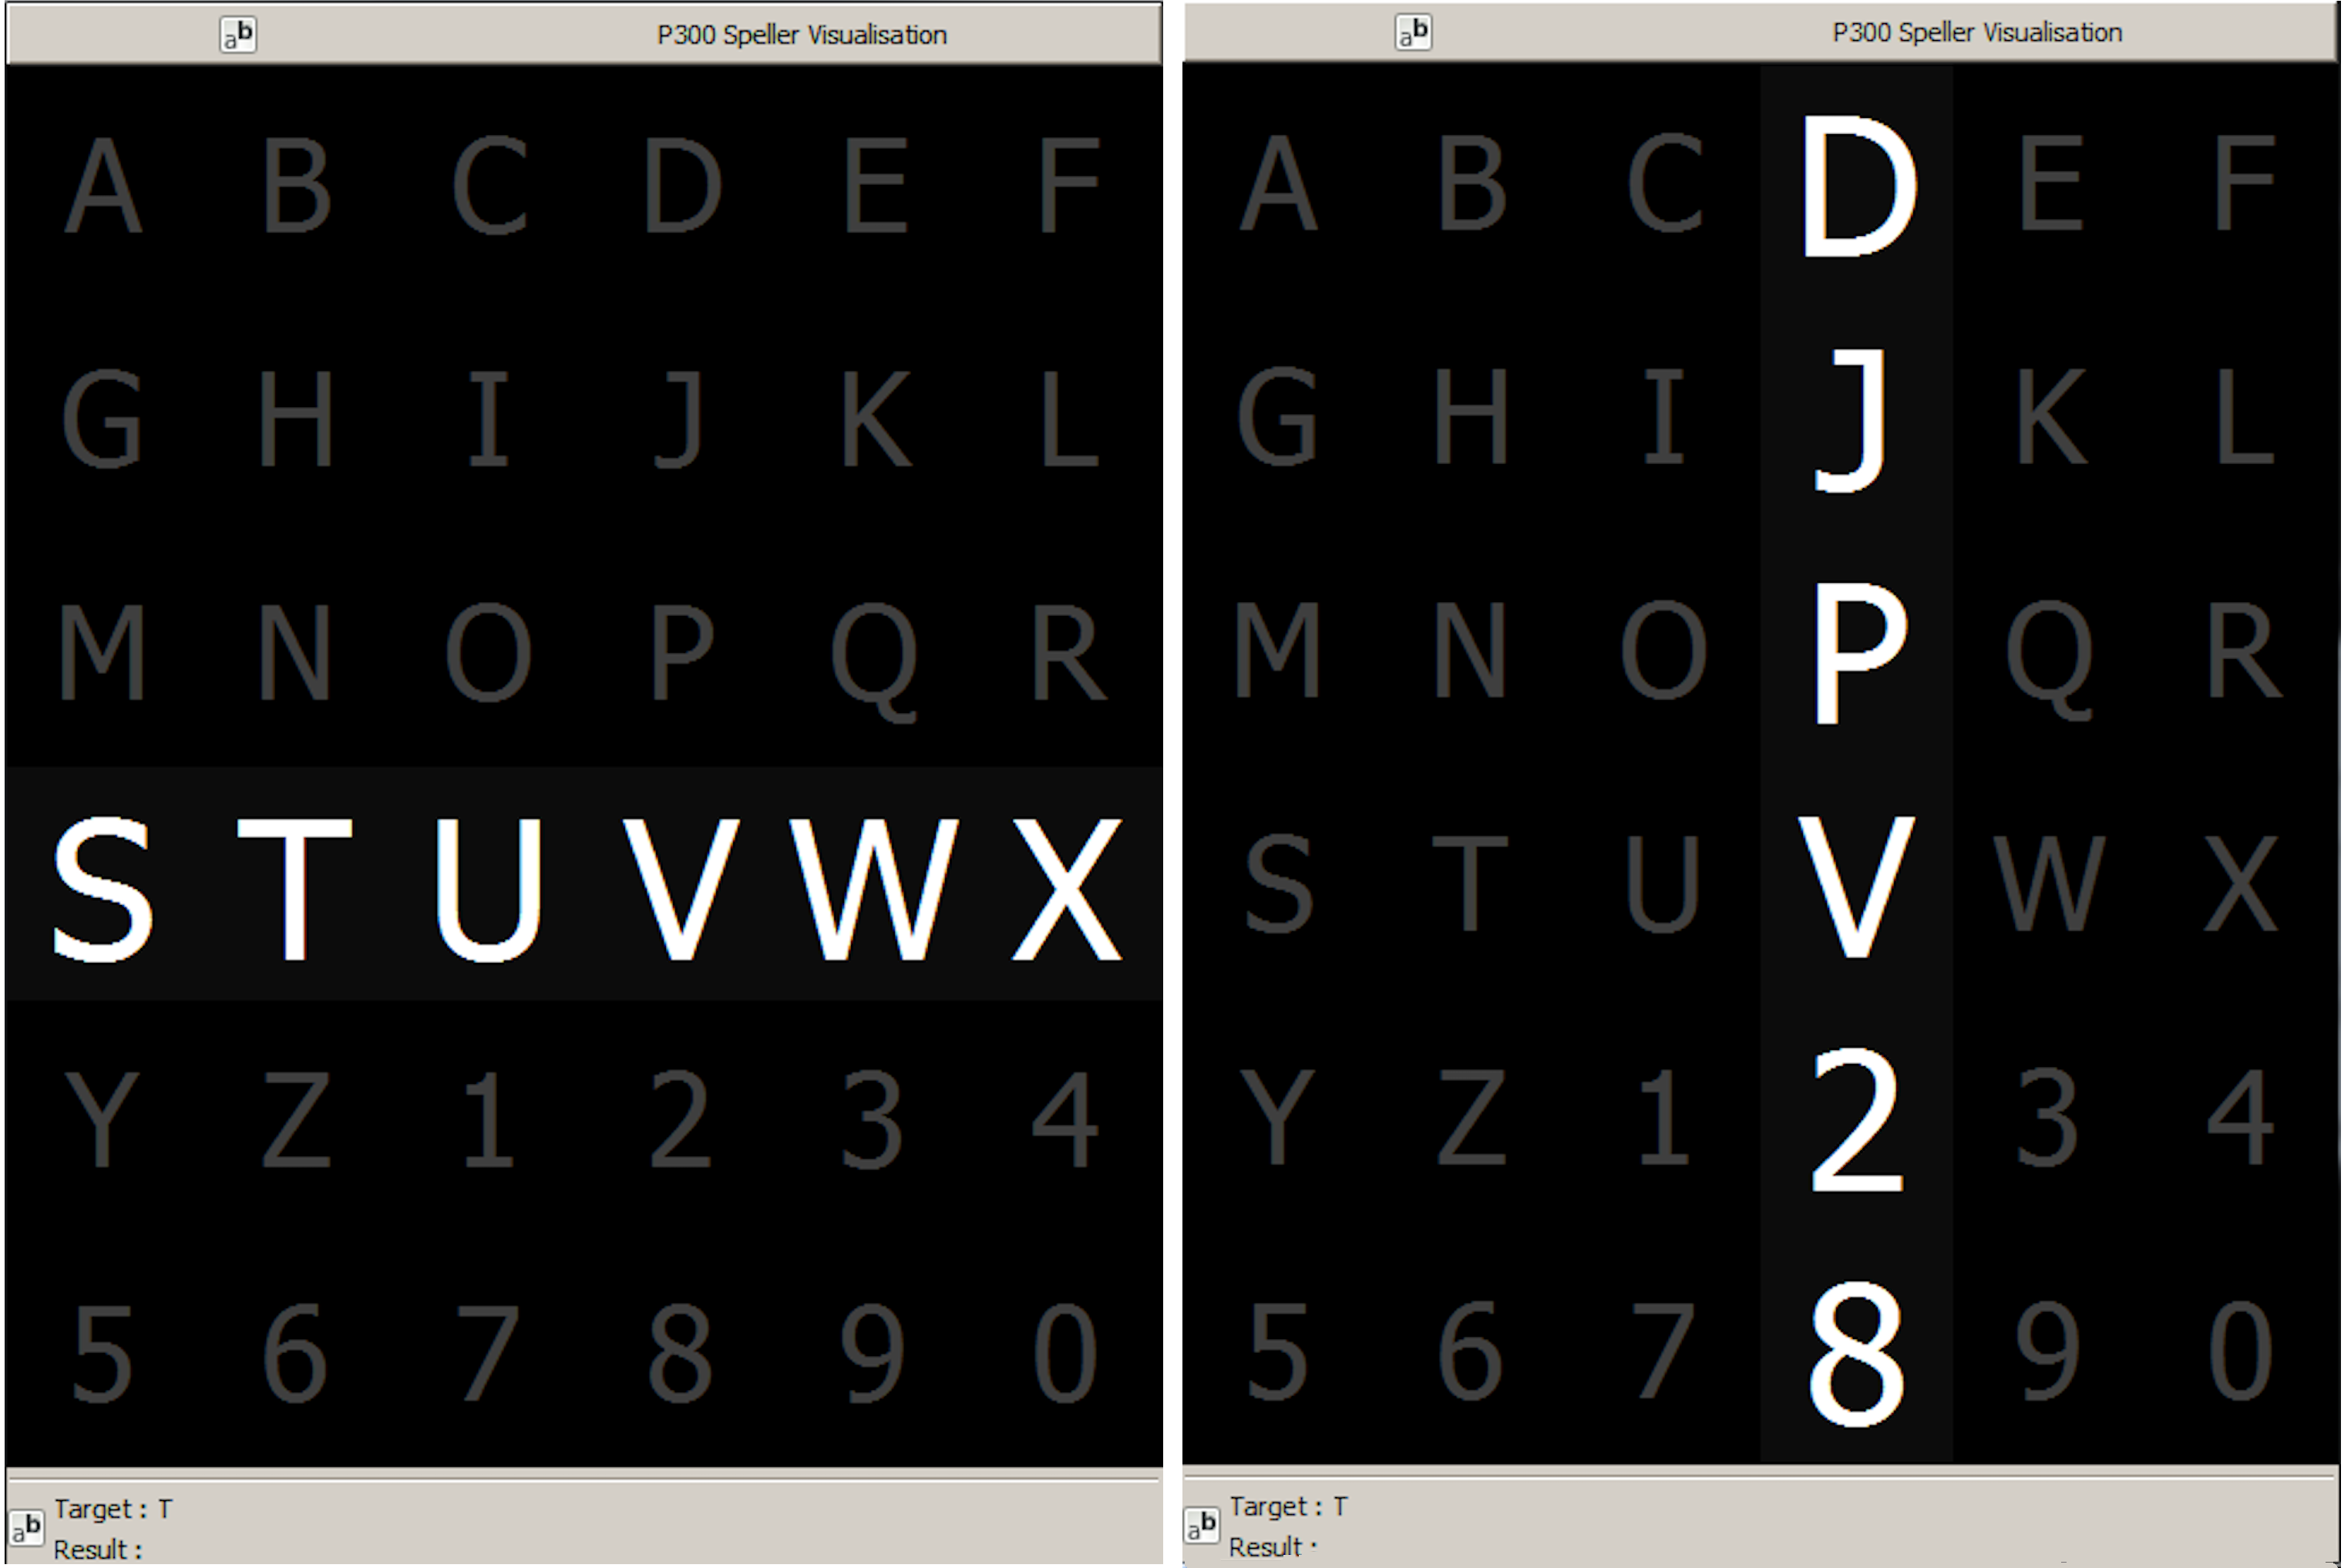
\includegraphics[width=15cm]{openvibep300matrix.png}
\caption{Example of the $6 \times 6$ Speller Matrix used in the study obtained from the OpenVibe software.  Rows and columns flash in random permutations.}
\label{fig:p300matrix}
\end{figure}

\begin{figure}[h!]
\centering
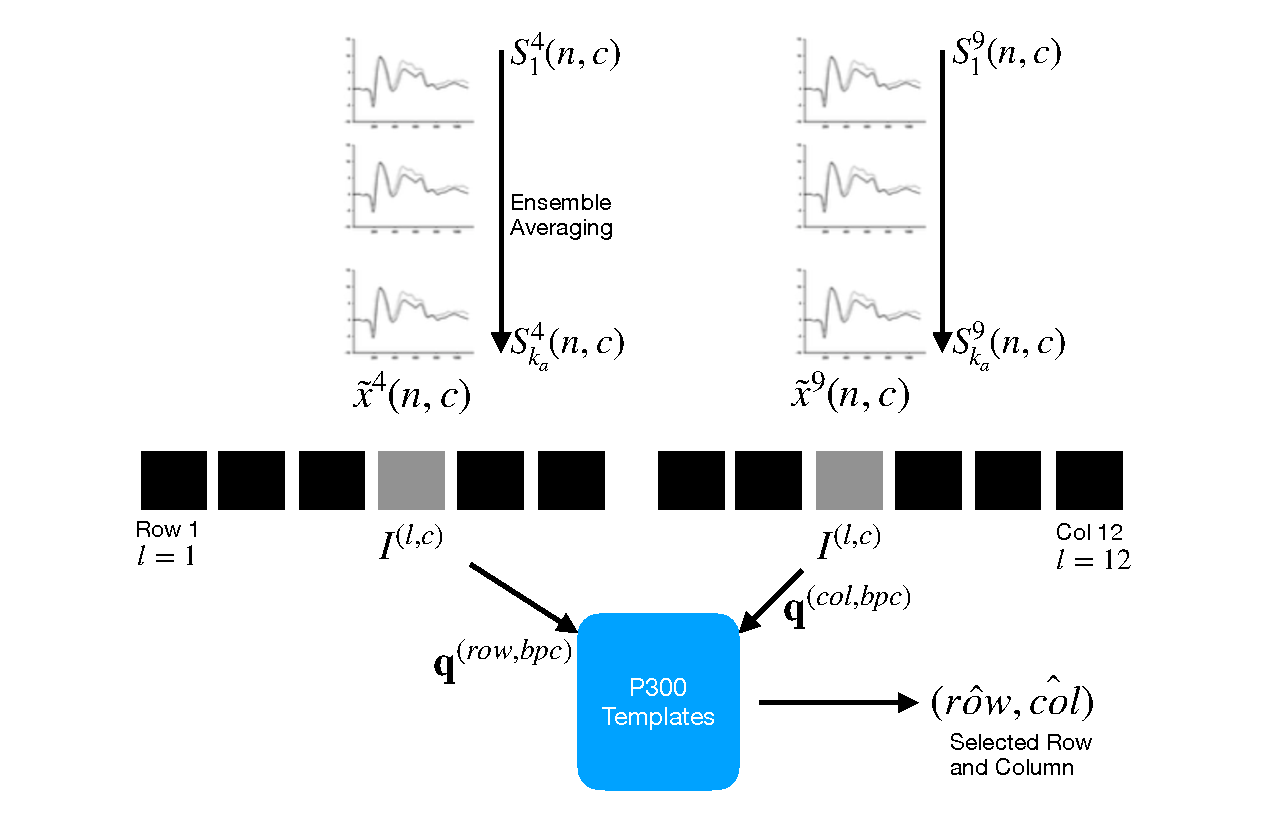
\includegraphics[width=15cm]{classificationgraph.pdf}
\caption{For each column and row, an averaged, standardized and scaled signal $\tilde{x}^l(n,c)$ is obtained from the segments $S_i^l$  corresponding to the $k_a$ intensification sequences with $ 1 \leq i \leq k_a $ and location $l$ varying between $1$ and $12$. From the averaged signal, the image $I^{(l,c)}$ of the signal plot is generated and each descriptor is computed.  By comparing each descriptor against the set of templates, the P300 ERP can be detected, and finally the desired letter from the matrix can be inferred.}
\label{fig:classification}
\end{figure}

\begin{figure}[h!]
\centering
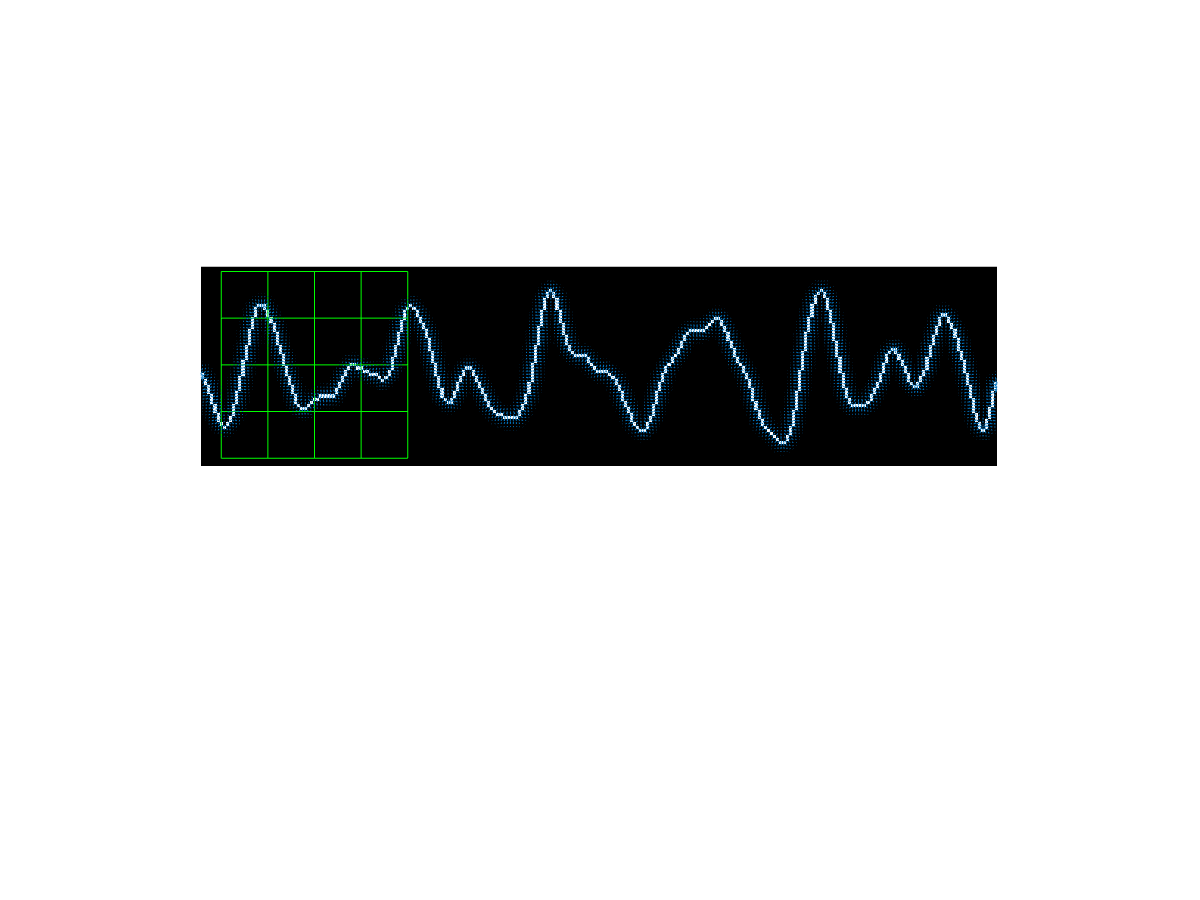
\includegraphics[width=16cm]{gradients.png}\label{samplegradients}
\caption{ (A) Example of a plot of the signal, a keypoint and the corresponding patch. (B) A scheme of the orientation's histogram computation.  Only the upper-left four blocks are visible.  The first eight orientations of the first block, are labeled from $1$ to $8$ clockwise. The orientation of the second block $ B_{1,2} $ is labeled from $9$ to $16$.  This labeling continues left-to-right, up-down until the eight orientations for all the sixteen blocks are assigned. They form the corresponding descriptor of $128$ coordinates.  The length of each arrow represent the value of the histogram on each direction for each block. (C) Vector field of oriented gradients.  Each pixel is assigned an orientation and magnitude calculated  using finite differences. }
\label{fig:sampledescriptor}
\end{figure}

\begin{figure}[h!]
\centering
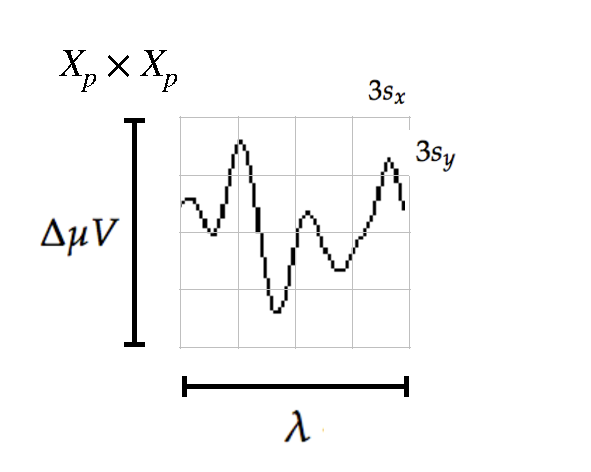
\includegraphics[width=10cm]{patchgeometry.pdf}
\caption{The scale of local patch is selected in order to capture the whole transient event.  The size of the patch is $X_p \times X_p$ pixels. The vertical size consists of $4$ blocks of size $3 s_y$ pixels which is high enough as to contain the signal $\Delta  \mu V $, the peak-to-peak amplitude of the transient event. The horizontal size includes $4$ blocks  of $3 s_x$ and covers the entire duration in seconds of the transient signal event, $ \lambda $.   }
\label{fig:patchgeometry}
\end{figure}

\begin{figure}[h!]
\centering
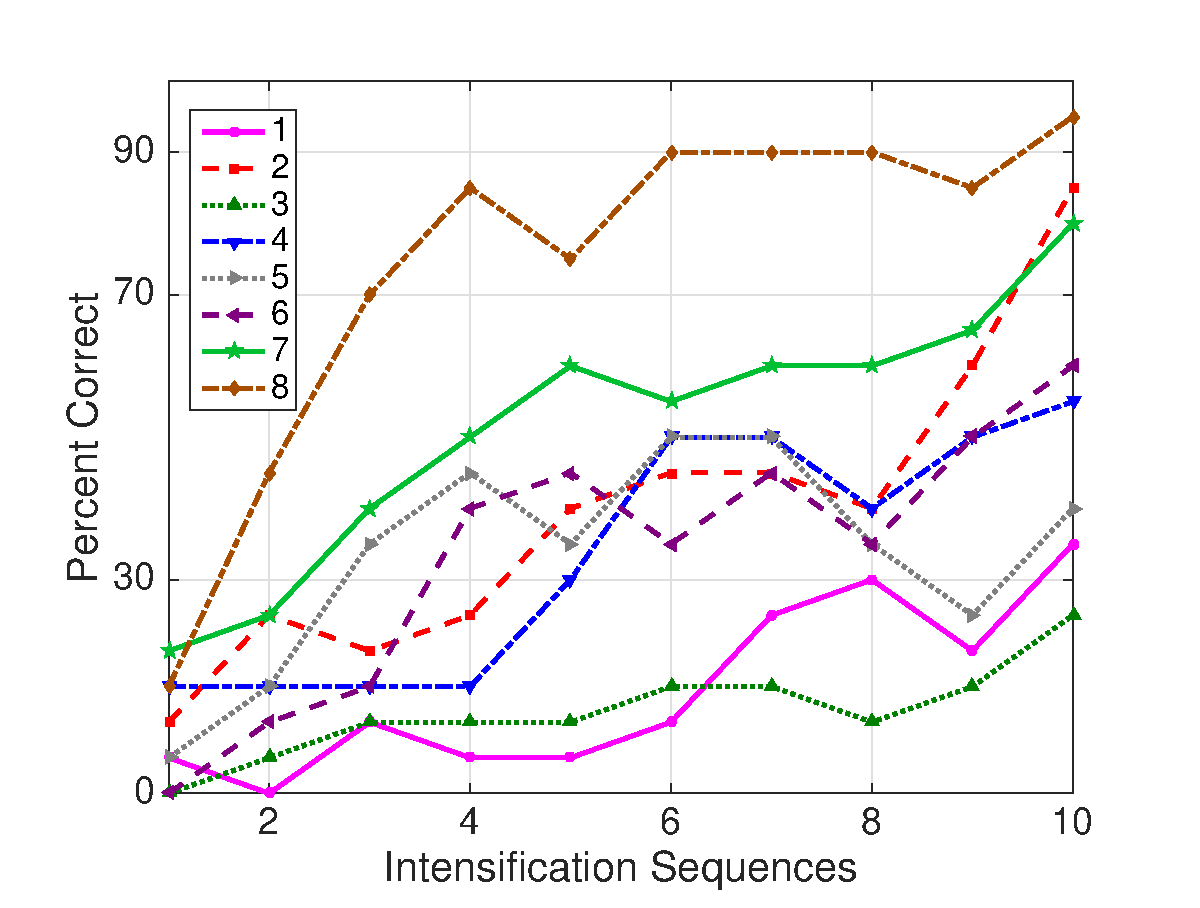
\includegraphics[width=10cm]{performance.eps}
\caption{Performance curves for the eight subjects included in the dataset of ALS patients.  Three out of eight subjects achieved the necessary performance to implement a valid P300 speller.}
\label{fig:performance}
\end{figure}


\begin{figure}[h!]
\centering
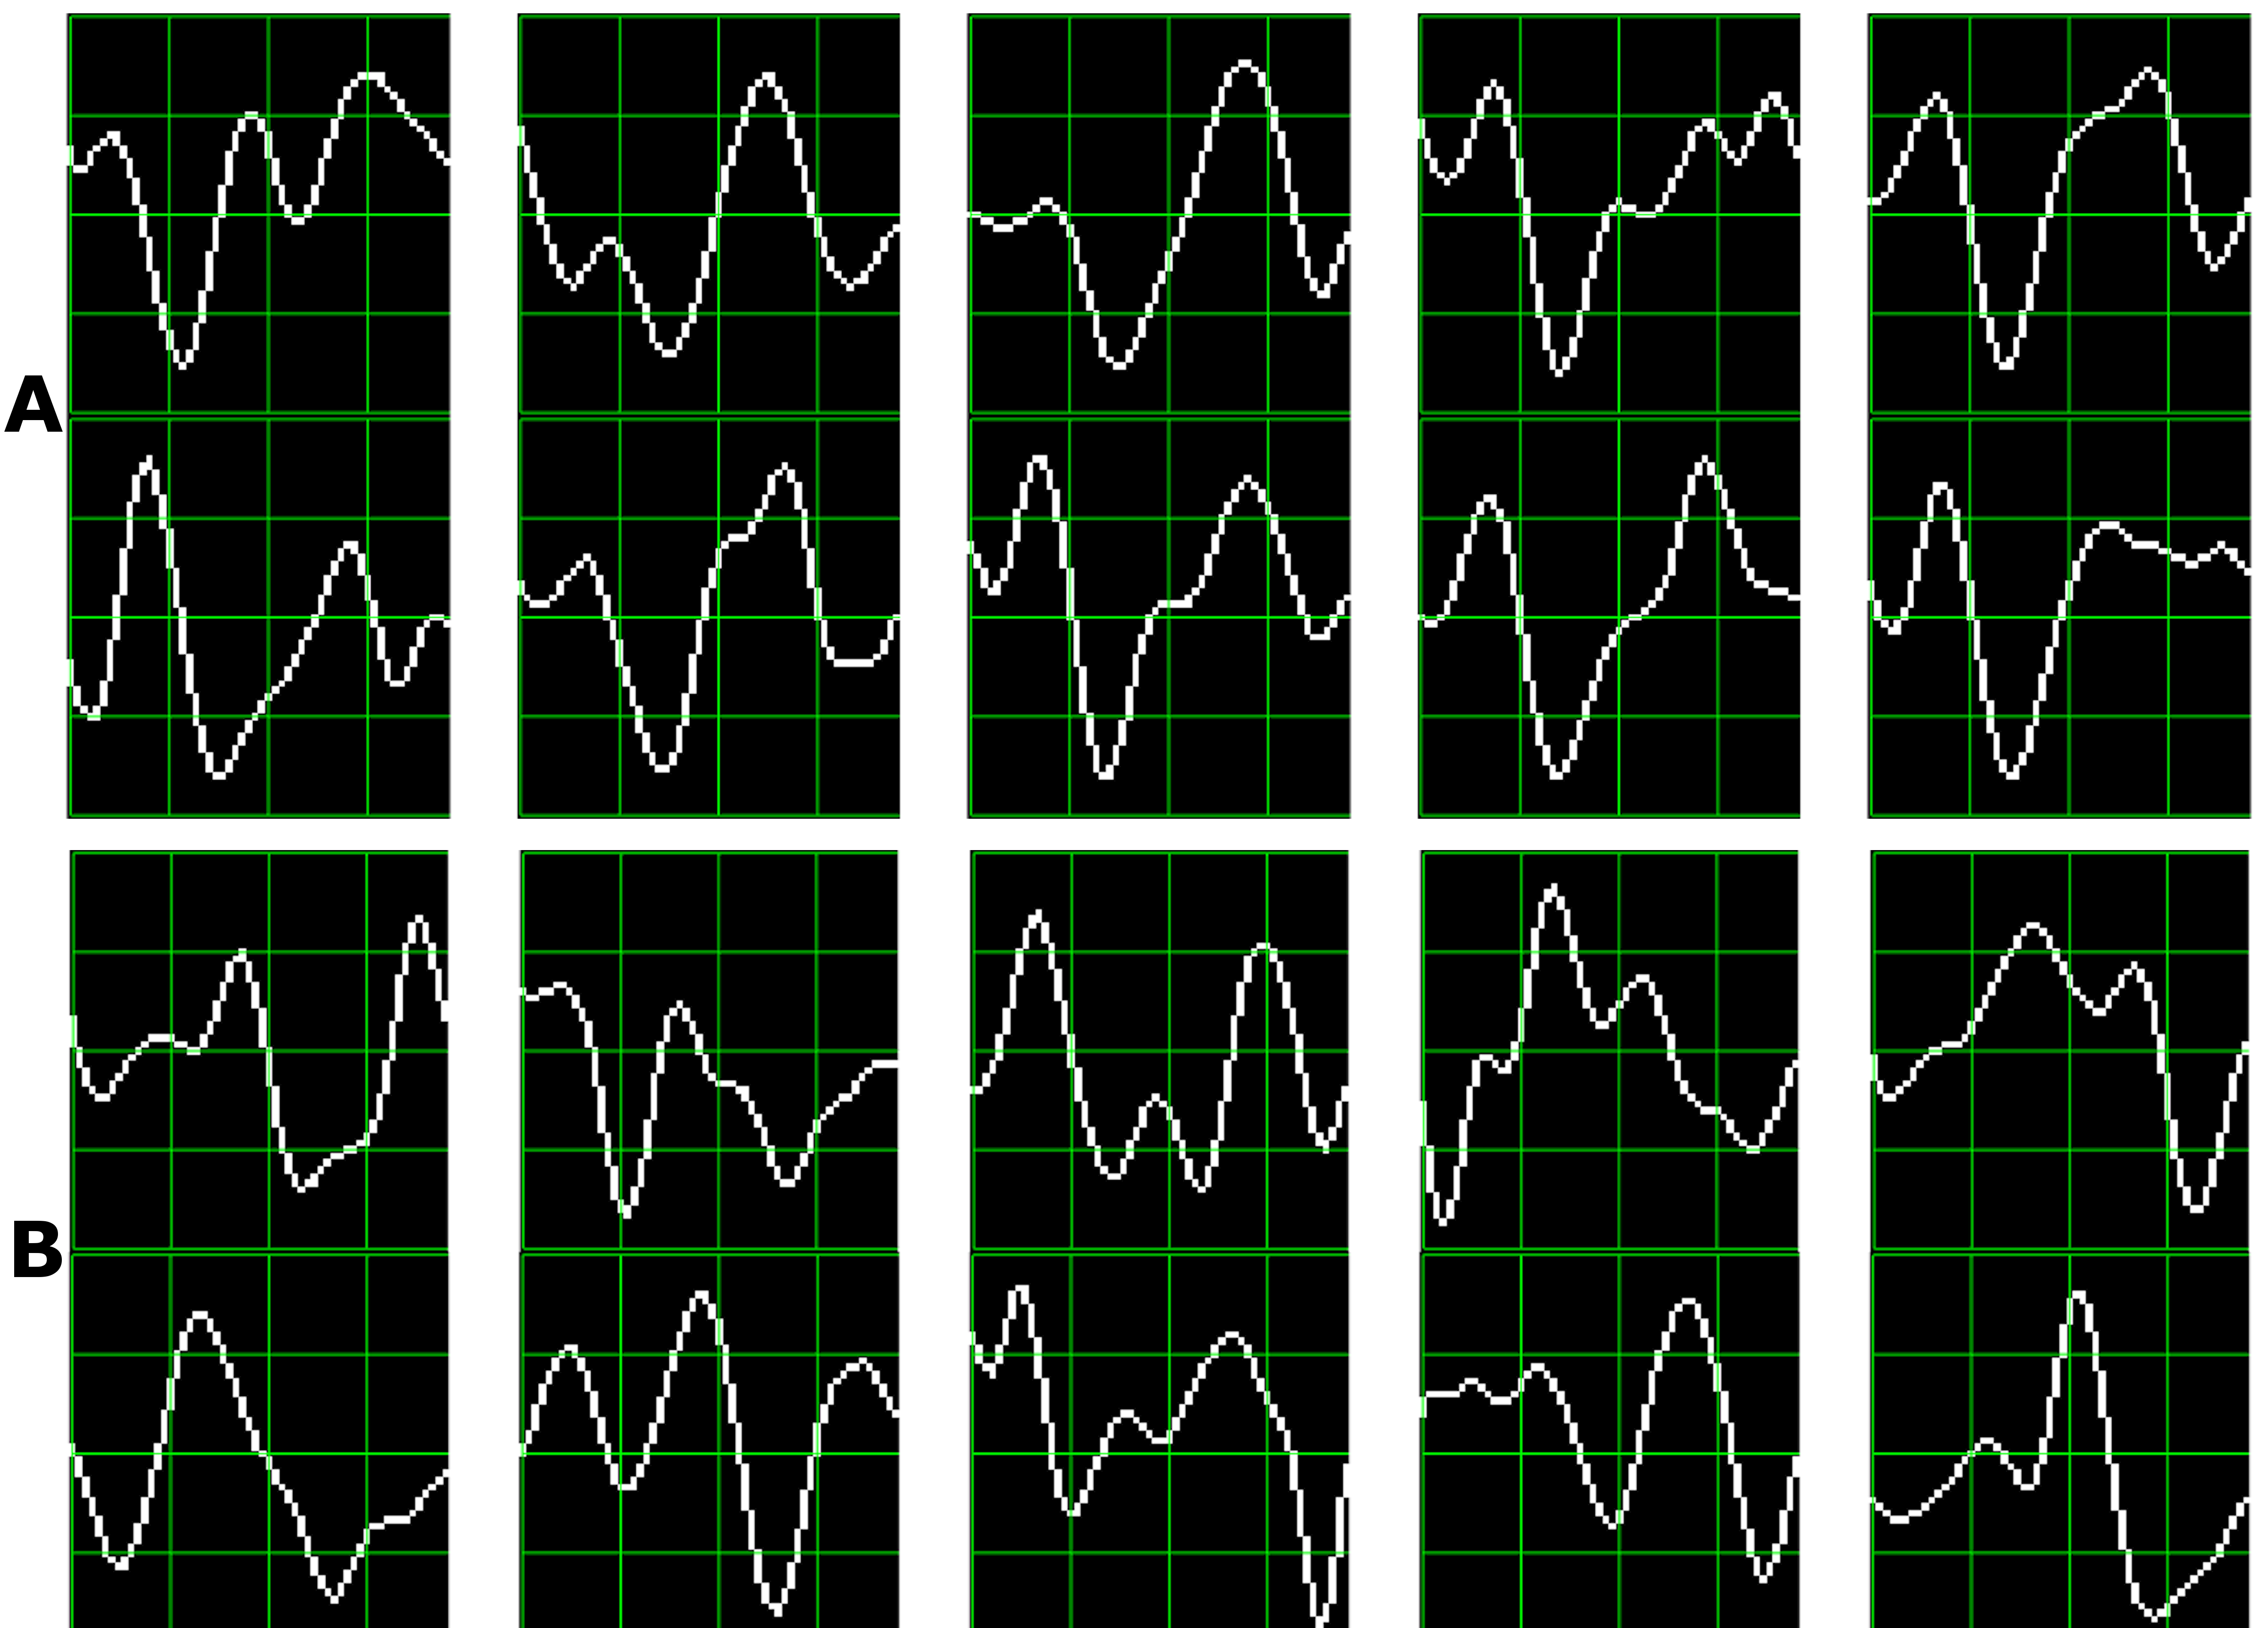
\includegraphics[width=15cm]{subject.png}\label{subject8}
\caption{Ten sample P300 template patches for subjects 8 (A) and 3 (B) of the ALS Dataset.  Downward deflection is positive polarity. }
\label{fig:p300templates}
\end{figure}

\end{document}
